\ylDisplay{Nõguslääts} % Ülesande nimi
{Tundmatu autor} % Autor
{piirkonnavoor} % Voor
{2016} % Aasta
{P 7} % Ülesande nr.
{3} % Raskustase
{
% Teema: Valgusõpetus
\ifStatement
Punkt $A$ ja selle kujutis $A'$ asuvad läätse optilisest peateljest vastavalt $3$ cm ja $1$ cm kaugusel. Punkti $A$ ja selle kujutise kaugus mööda optilist peatelge on $10$ cm. Kui suur on läätse fookuskaugus, kui tegemist on nõgusläätsega?
\fi

\ifHint
Ülesande lahendamiseks konstrueeri nõugusläätsesüsteemi kujutav joonis, kus tekkiv kujutis on näiline, samapidine ja vähendatud. Fookuskauguse leidmisel saad kasutada kolmnurkade sarnasust.
\fi


\ifSolution
\begin{center}
	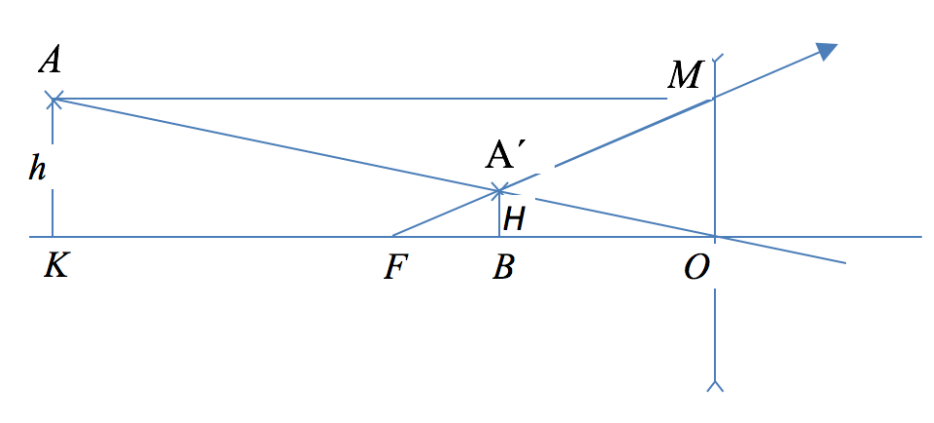
\includegraphics[width=0.5\linewidth]{2016-v2p-07-lah.PNG}
\end{center}
Näha on, et $AK = OM = h$. \\
Tähistame $A^\prime B = H$, $KO = a$, $FO = f$ ja $BO = k$. \\
Kolmnurkade $\triangle FMO$ ja $\triangle FBA^\prime$ sarnasusest selgub, et 
\begin{center}
$\cfrac{h}{H} = \cfrac{OF}{FB} = \cfrac{f}{f - k}$,
\end{center}
millest $hf - hk = H f$, millest
\begin{center}
$f = \cfrac{hk}{h - H}$.
\end{center}
Et arvutada fookuskaugust tuleb teada kujutise kaugust. Kolmnurkade $\triangle AKO$ ning $\triangle BOA^\prime$ sarnasusest selgub, et
\begin{center}
$\cfrac{h}{H} = \cfrac{a}{k}$.
\end{center}
Asendades $a = 10 + k$ saame, et
\begin{center}
$\cfrac{h}{H}$ $= \cfrac{10 + k}{k}$ ning $k = \cfrac{10H}{h - H} = 5$ $cm$
\end{center}
ning
\begin{center}
$f = \cfrac{hk}{h - H} = 7,5$ $cm$.
\end{center}
\fi
}